\documentclass{article}
\usepackage[utf8]{inputenc}

% a single package needed for the plot to work
\usepackage{pgfplots}

% suppress compatibility warning
\pgfplotsset{compat=1.8}

% format reference hyperlinks
\usepackage{hyperref}
\usepackage{xcolor}
\hypersetup{
    colorlinks,
    linkcolor={blue!100!black},
    citecolor={blue!100!black},
    urlcolor={blue!100!black}
}


\title{Tikz Plot Reproduction}
\author{Kenan Tang}
\date{July 2022}

\begin{document}

\maketitle

\section{The Plot}

From the error count results in Figure \ref{fig:results}, we see that \textbf{GTT makes fewer Missing Template errors than DyGIE++ on the MUC-4 dataset} (86 vs. 97).

\begin{figure}[!htbp]
    \centering
    
    % fit to page width
    \resizebox{\columnwidth}{!}{%

        % This file was PARTLY created with tikzplotlib v0.10.1.
        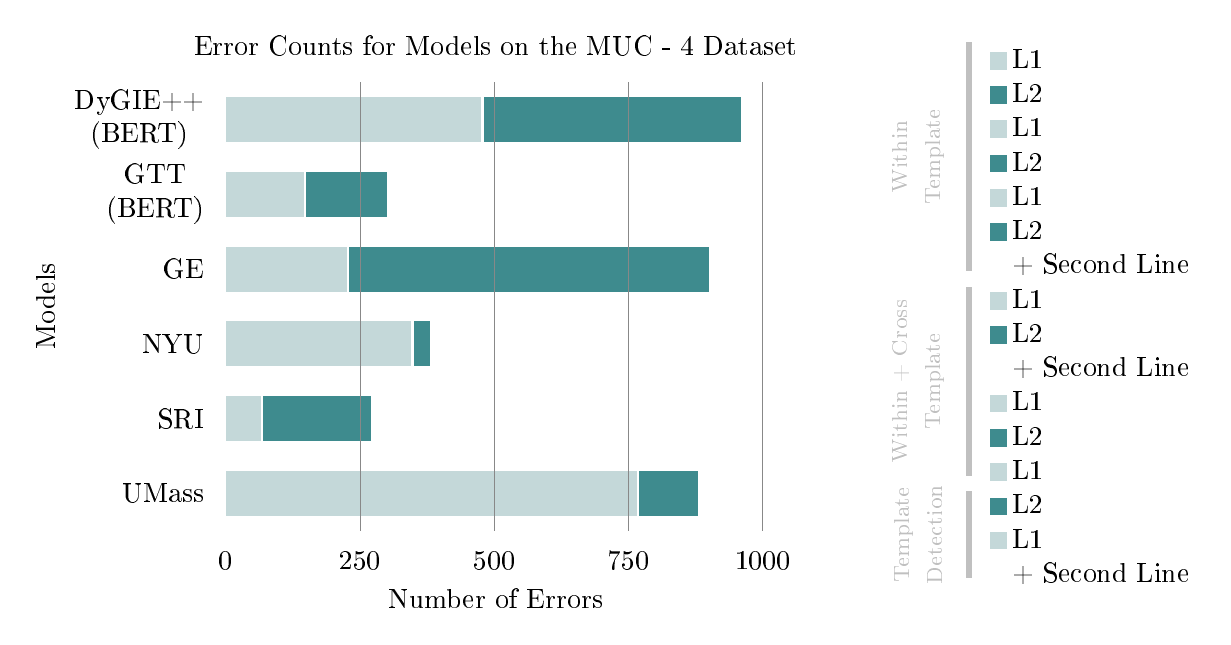
\begin{tikzpicture}
        
        % put this after begin tikzpicture, so that it applies to all text
        \usefont{T1}{custom}{m}{n}
        
        % define colors, picked from the original paper
        \definecolor{gray136}{RGB}{136,136,136}
        \definecolor{gray192}{RGB}{192,192,192}
        \definecolor{green196}{RGB}{196,216,217}
        \definecolor{green62}{RGB}{62,139,142}
        
        \begin{axis}[
        axis line style={draw=none}, % remove border box
        tick style={draw=none}, % remove short-line ticks
        legend cell align={left},
        legend style={
          at={(1.4,1.1)}, % to the right of the plot
          anchor=north west,
          draw=none, % no border
          align=left,  % allow multiple lines in legend
          mark options={mark size=3pt} % slightly larger marker, default is 2pt
        },
        tick align=outside,
        tick pos=left,
        title={Error Counts for Models on the MUC - 4 Dataset},
        xlabel={Number of Errors},
        xmin=0, xmax=1005, % leave space for the last line, cannot be exactly 1000
        xtick={0, 250, 500, 750, 1000},
        y dir=reverse, % top to bottom
        ylabel={Models},
        ymin=-0.5, ymax=5.5,
        ytick={0,1,2,3,4,5},
        yticklabel style={align=center}, % provide align, so that line-breaks work
        yticklabels={DyGIE++\\(BERT), GTT\\(BERT), GE, NYU, SRI, UMass},
        tick label style={/pgf/number format/assume math mode}, % assume math mode so that the font applies to tick numbers as well
        /pgf/number format/.cd, use comma, 1000 sep={}, % remove comma separation for 1,000
        ]
        
        % all legends, filled square*, the same color for fill and draw
        \addlegendimage{only marks, mark=square*, fill=green196, draw=green196}
        \addlegendentry{L1}
        \addlegendimage{only marks, mark=square*, fill=green62, draw=green62}
        \addlegendentry{L2}
        \addlegendimage{only marks, mark=square*, fill=green196, draw=green196}
        \addlegendentry{L1}
        \addlegendimage{only marks, mark=square*, fill=green62, draw=green62}
        \addlegendentry{L2}
        \addlegendimage{only marks, mark=square*, fill=green196, draw=green196}
        \addlegendentry{L1}
        \addlegendimage{only marks, mark=square*, fill=green62, draw=green62}
        \addlegendentry{L2}
        \addlegendimage{only marks, opacity=0} % place holder
        \addlegendentry{+ Second Line} % better than line-break
        \addlegendimage{only marks, mark=square*, fill=green196, draw=green196}
        \addlegendentry{L1}
        \addlegendimage{only marks, mark=square*, fill=green62, draw=green62}
        \addlegendentry{L2}
        \addlegendimage{only marks, opacity=0} % place holder
        \addlegendentry{+ Second Line} % better than line-break
        \addlegendimage{only marks, mark=square*, fill=green196, draw=green196}
        \addlegendentry{L1}
        \addlegendimage{only marks, mark=square*, fill=green62, draw=green62}
        \addlegendentry{L2}
        \addlegendimage{only marks, mark=square*, fill=green196, draw=green196}
        \addlegendentry{L1}
        \addlegendimage{only marks, mark=square*, fill=green62, draw=green62}
        \addlegendentry{L2}
        \addlegendimage{only marks, mark=square*, fill=green196, draw=green196}
        \addlegendentry{L1}
        \addlegendimage{only marks, opacity=0} % place holder
        \addlegendentry{+ Second Line} % better than line-break
        
        % the bars, manually added gaps (480-475=5) between bars
        \draw[draw=none,fill=green196] (axis cs:0,-0.3) rectangle (axis cs:475,0.3);
        \draw[draw=none,fill=green62] (axis cs:480,-0.3) rectangle (axis cs:960,0.3);
        \draw[draw=none,fill=green196] (axis cs:0,0.7) rectangle (axis cs:145,1.3);
        \draw[draw=none,fill=green62] (axis cs:150,0.7) rectangle (axis cs:300,1.3);
        \draw[draw=none,fill=green196] (axis cs:0,1.7) rectangle (axis cs:225,2.3);
        \draw[draw=none,fill=green62] (axis cs:230,1.7) rectangle (axis cs:900,2.3);
        \draw[draw=none,fill=green196] (axis cs:0,2.7) rectangle (axis cs:345,3.3);
        \draw[draw=none,fill=green62] (axis cs:350,2.7) rectangle (axis cs:380,3.3);
        \draw[draw=none,fill=green196] (axis cs:0,3.7) rectangle (axis cs:65,4.3);
        \draw[draw=none,fill=green62] (axis cs:70,3.7) rectangle (axis cs:270,4.3);
        \draw[draw=none,fill=green196] (axis cs:0,4.7) rectangle (axis cs:765,5.3);
        \draw[draw=none,fill=green62] (axis cs:770,4.7) rectangle (axis cs:880,5.3);
        
        % Instead of ticks, draw these vertical lines, after the bars have been drawn. The plot in the original paper has some inconsistencies in the order of drawing bars and these lines, so that lines do not always appear above bars.
        \addplot[mark=none, gray136] coordinates {(250,-0.5) (250,5.5)};
        \addplot[mark=none, gray136] coordinates {(500,-0.5) (500,5.5)};
        \addplot[mark=none, gray136] coordinates {(750,-0.5) (750,5.5)};
        \addplot[mark=none, gray136] coordinates {(1000,-0.5) (1000,5.5)};
        
        \end{axis}
        
        % Legend categories. The spacing between rectangles are kept the same here (0.2), but not in the original paper. 
        \draw[draw=none,fill=gray192] (9.4, 3.3) rectangle (9.48, 6.2);
        \draw[draw=none,fill=gray192] (9.4, 0.7) rectangle (9.48, 3.1);
        \draw[draw=none,fill=gray192] (9.4, -0.6) rectangle (9.48, 0.5);
        
        \node[rotate=90, align=center, gray192] at (8.8, 4.75) {\footnotesize Within \\ \footnotesize Template}; % 4.75 = (3.3 + 6.2) / 2, use slightly smaller text
        \node[rotate=90, align=center, gray192] at (8.8, 1.9) {\footnotesize Within + Cross \\ \footnotesize Template};
        \node[rotate=90, align=center, gray192] at (8.8, -0.05) {\footnotesize Template \\ \footnotesize Detection};
        
        \end{tikzpicture}%
    }
    
    \caption{Automated Error Analysis Results (Error Counts) for Models on the MUC-4 dataset.}
    \label{fig:results}
\end{figure}

\end{document}
